\section{Preliminary Experiments}\label{sec:experiments}

\subsection{Experimental protocol}

The current draft uses the repository's existing synthetic benchmark suite as a controlled pilot study. The runs are generated from \path{paper_assets/configs/publication_suite.yaml} and cover three scenario families:

\begin{itemize}
  \item \textbf{Covariate-shift sweep}: varying shift severity in a binary tabular classification task.
  \item \textbf{Subgroup degradation}: hidden failure modes concentrated in minority or masked subgroups.
  \item \textbf{Selective shift}: abstention-based deployment policies under increasing shift.
\end{itemize}

Each scenario currently uses only two seeds in the committed artifact suite, so the results below are best read as a serious pilot rather than a final statistical study. They are still useful because they match the main objects of the theory: effective sample size, target calibration, worst-group gaps, and selective risk.

To make the scenarios concrete:
\begin{itemize}
  \item in the covariate-shift sweep, the same prediction task is kept fixed while the target covariates are moved farther away from the source covariates;
  \item in the subgroup benchmarks, failure is concentrated in one subgroup even when overall metrics remain moderate;
  \item in the selective benchmark, the model may reject low-confidence examples and we measure the risk on the accepted set.
\end{itemize}

\subsection{Key empirical patterns}

\begin{table}[t]
\centering
\caption{Preliminary benchmark summary extracted from the committed publication suite. These numbers are not the final experimental campaign; they are the current strongest evidence already present in the repository.}
\label{tab:pilot-summary}
\begin{tabular}{p{0.29\linewidth}p{0.17\linewidth}p{0.46\linewidth}}
\toprule
Scenario & Setting & Observation \\
\midrule
Covariate shift & severity $0.20$ & effective sample size $\approx 179.8$; raw target ECE $\approx 0.075$; recalibrated target ECE $\approx 0.064$ \\
Covariate shift & severity $1.40$ & effective sample size $\approx 60.9$; raw target ECE $\approx 0.064$; recalibrated target ECE $\approx 0.057$ \\
Masked subgroup shift & audit baseline & worst-group accuracy gap $\approx 0.137$; worst-group ECE gap $\approx 0.182$ \\
Minority subgroup degradation & audit baseline & worst-group accuracy gap $\approx 0.140$; worst-group ECE gap $\approx 0.217$ \\
Selective shift & severity $0.40$ & weighted confidence abstention keeps coverage $\approx 0.707$ with target risk reduction $\approx 0.079$ and selective ECE $\approx 0.070$ \\
Selective shift & severity $1.00$ & weighted confidence abstention keeps coverage $\approx 0.759$ with target risk reduction $\approx 0.061$ and selective ECE $\approx 0.084$ \\
\bottomrule
\end{tabular}
\end{table}

\paragraph{Effective sample size degrades as shift severity increases.}
The covariate-shift benchmark exhibits a clear collapse in effective sample size, from roughly $180$ at severity $0.20$ to roughly $61$ at severity $1.40$. This matches \cref{thm:uniform}: even if weighted transport is valid in principle, the estimation problem becomes harder when a few source points carry most of the weight.

\paragraph{Aggregate target error can look moderate while worst-group gaps are large.}
In the hidden subgroup scenarios, the subgroup-audit baseline reports worst-group ECE gaps of about $0.182$ and $0.217$, together with worst-group accuracy gaps around $0.14$. In simple terms, the average target metric looks much better than the worst affected subgroup. This is exactly the hidden-failure phenomenon formalized earlier.

\paragraph{Selective policies improve accepted-set averages but require subgroup-aware interpretation.}
In the selective-shift pilot, weighted and recalibrated abstention policies retain roughly $71\%$ to $76\%$ coverage while reducing target selective risk. The weighted policy also achieves better accepted-set calibration than the recalibrated confidence baseline at both severities in the committed suite. The lesson is simple: abstention can help, but it should still be evaluated with subgroup-aware target metrics.

\begin{figure}[t]
\centering
\begin{subfigure}{0.48\linewidth}
  \centering
  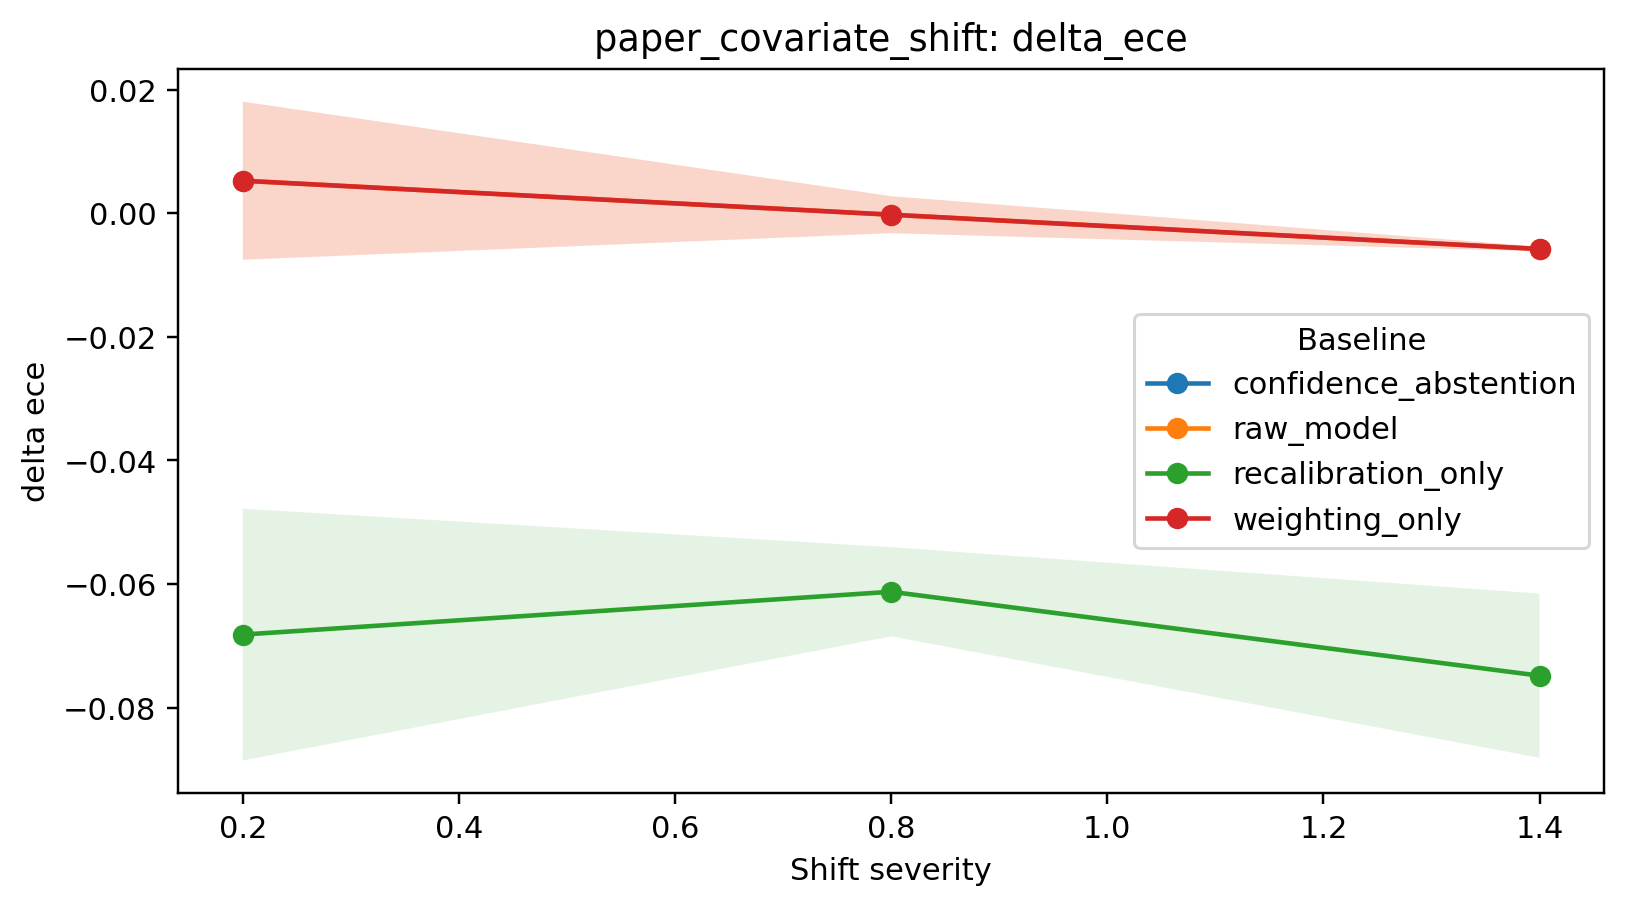
\includegraphics[width=\linewidth]{../paper_assets/generated/publication_suite/paper_covariate_shift/figures/paper_covariate_shift_delta_ece.png}
  \caption{Calibration change across covariate-shift severity.}
  \label{fig:covariate-ece}
\end{subfigure}
\hfill
\begin{subfigure}{0.48\linewidth}
  \centering
  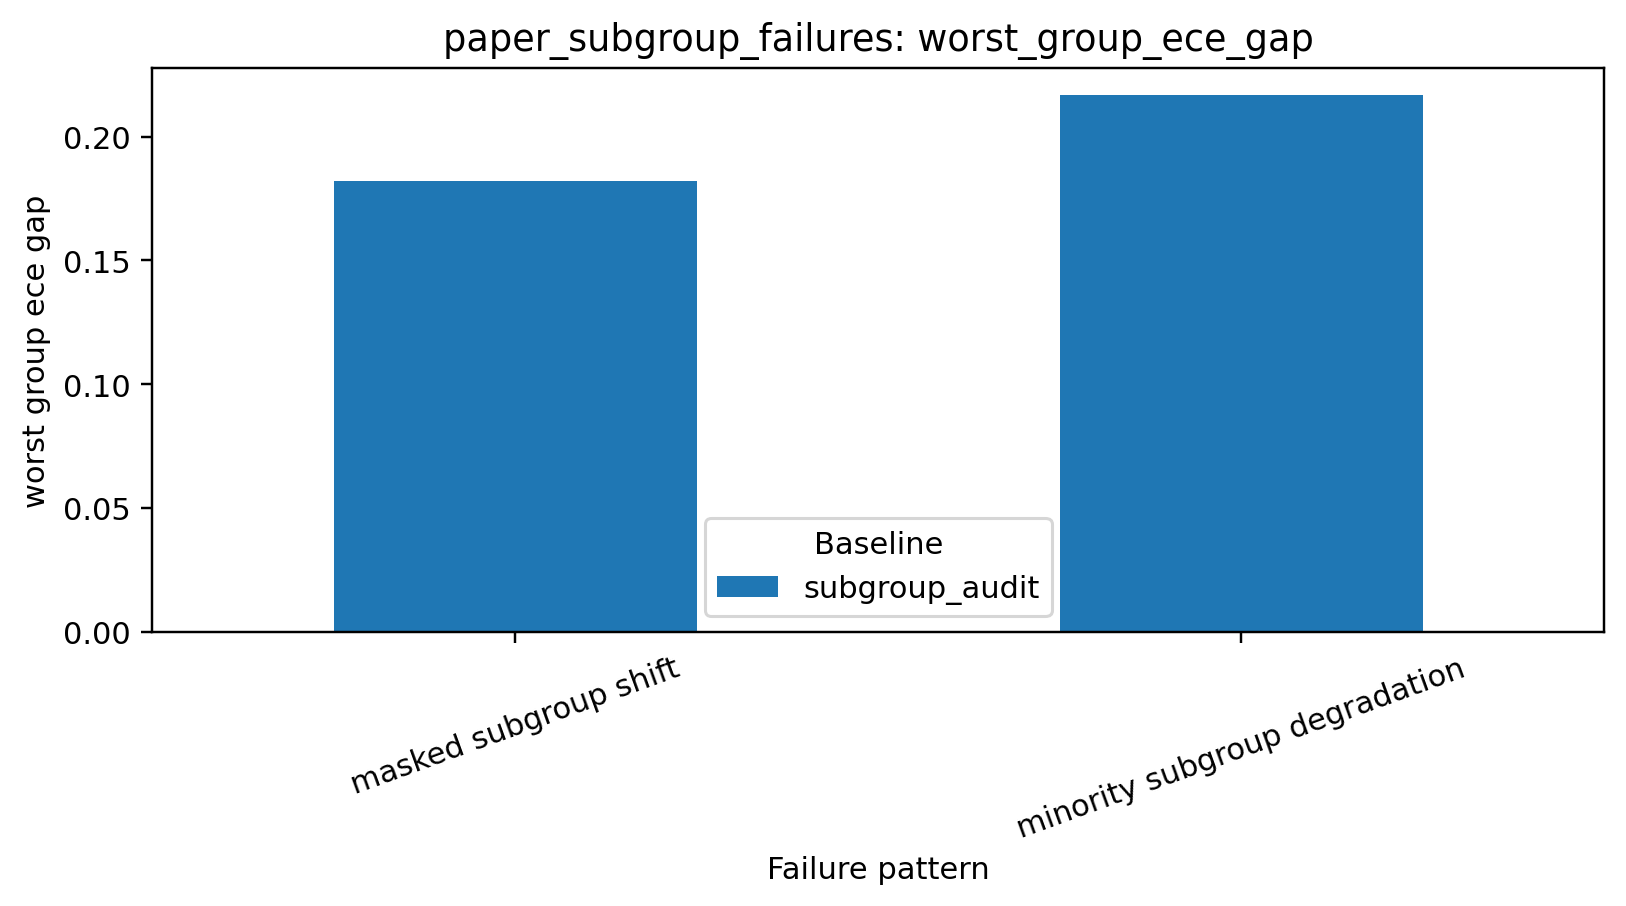
\includegraphics[width=\linewidth]{../paper_assets/generated/publication_suite/paper_subgroup_failures/figures/paper_subgroup_failures_worst_group_ece_gap.png}
  \caption{Worst-group calibration gap in hidden-failure scenarios.}
  \label{fig:subgroup-ece}
\end{subfigure}
\caption{Two pilot figures from the repository's benchmark suite. The left panel shows how a calibration-oriented metric changes as shift severity increases. The right panel shows that worst-group ECE gaps stay large in subgroup-failure scenarios.}
\label{fig:pilot-main}
\end{figure}

\begin{figure}[t]
\centering
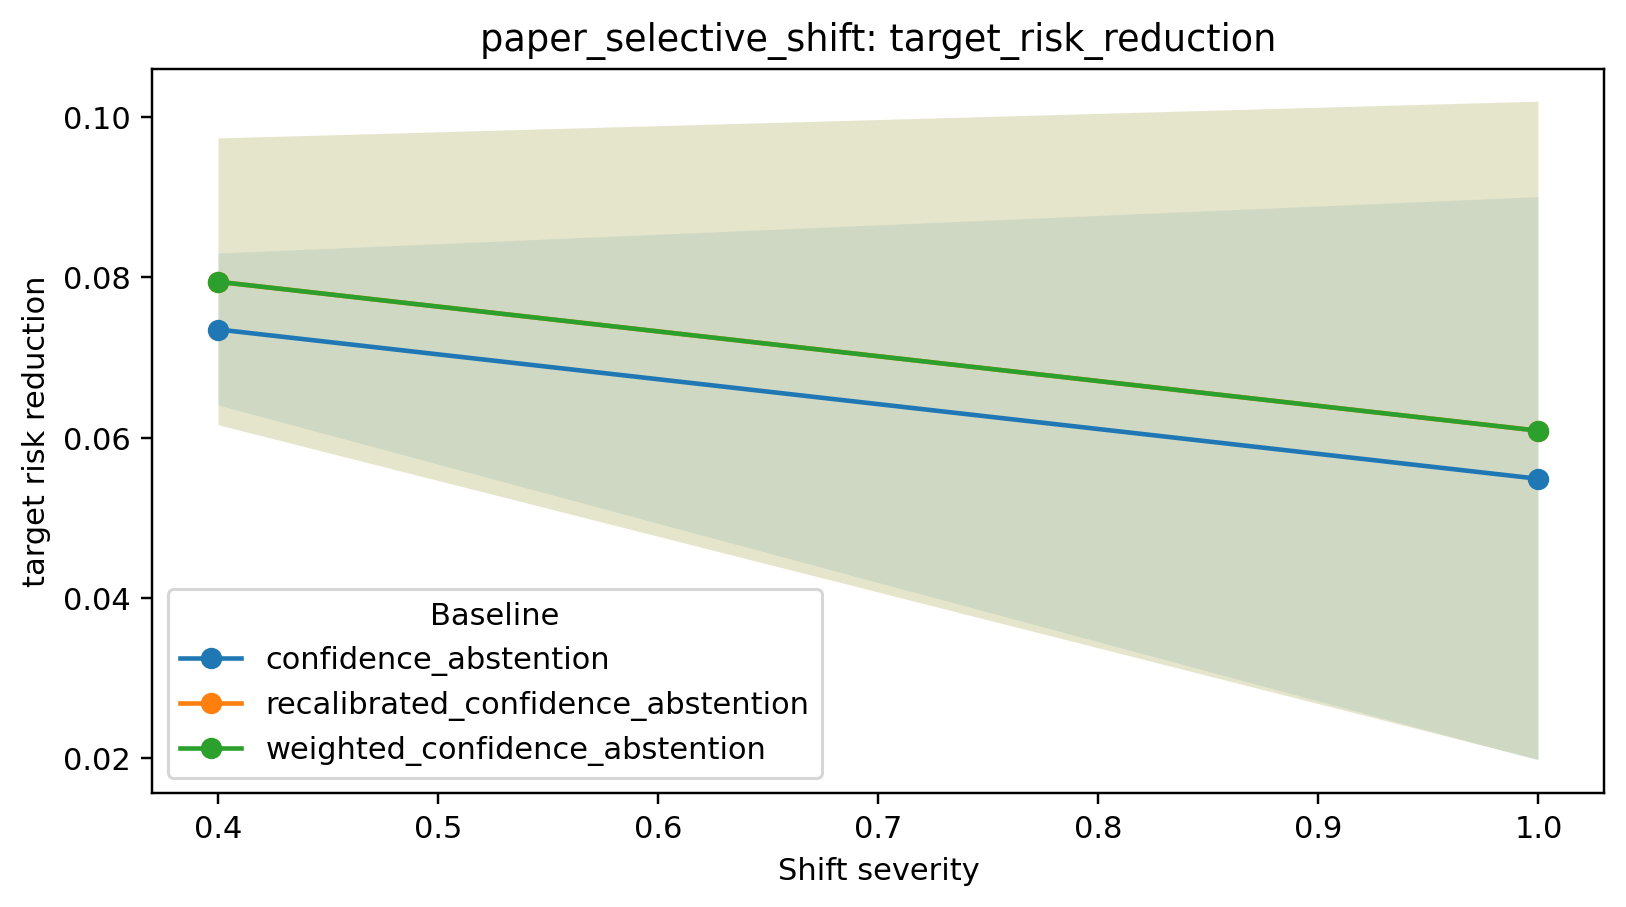
\includegraphics[width=0.66\linewidth]{../paper_assets/generated/publication_suite/paper_selective_shift/figures/paper_selective_shift_target_risk_reduction.png}
\caption{Target risk reduction in the selective-shift benchmark. Even when abstention improves average accepted-set risk, it should still be read together with subgroup rejection behavior and accepted-set calibration.}
\label{fig:selective-risk}
\end{figure}

\subsection{How the final paper should extend these experiments}

The current pilot is enough to support the theoretical framing, but not enough for a finished preprint. The final experimental section should strengthen the manuscript in four ways:

\begin{enumerate}
  \item increase the number of seeds so uncertainty intervals become meaningful;
  \item add ablations on density-ratio quality and explicit overlap violation;
  \item vary subgroup family complexity, from single features to intersectional slices;
  \item include at least one non-synthetic or semi-real tabular benchmark where subgroup prevalence shift is operationally plausible.
\end{enumerate}

These extensions would turn the current manuscript from a strong theory draft with executable evidence into a much more convincing empirical paper.
